\section{Experiments}

In this section, we evaluate the performance of state-of-the-art (SOTA) methods in both English and Chinese. The experimental results indicate that OmniEduBench remains a competitive benchmark.

\subsection{Experimental Setup}

\begin{table}[t]
    \centering
    \caption{Zero-shot average accuracy (\%) across six categories in the \textbf{knowledge}. The highest accuracy is \textbf{bold}, and the second highest is \underline{underlined}. More results are provided in the Appendix.}
    \vspace{0.2mm}
    \resizebox{0.99\textwidth}{!}{
        \begin{tabular}{lccc|cccccc|c}
            \toprule
            \textbf{Model} & \textbf{Parameters} & \textbf{Access} & \textbf{Creator} & \textbf{FD} & \textbf{HH} & \textbf{SSEM} & \textbf{LP} & \textbf{MH} & \textbf{IIS} & \textbf{Average} \\ \midrule
            Qwen3  & 8B & Weights & Alibaba & 53.02 & 38.53 & 36.58 & 30.17 & 36.71 & 37.75 & 43.86 \\
            Qwen3   & 14B & Weights & Alibaba & 36.32 & 36.78 & 35.12 & 27.29 & 36.82 & 35.67 & 35.62 \\
            MuduoLLM & 14B & Weights & BNU \& TAL & 28.20 & 40.82 & 32.99 & 36.15 & 39.11 & 31.40 & 33.68 \\
            QwQ   & 32B & Weights & Alibaba & \underline{61.25} & 48.51 & 42.24 & \underline{49.90} & 55.01 & 47.26 & \underline{53.87} \\
            Seed-OSS     & 36B & Weights & ByteDance & 48.81 & \underline{50.14} & \underline{45.34} & 48.66 & \textbf{61.00} & \underline{49.56} & 49.53 \\
            Qwen2.5 & 72B & Weights & Alibaba & 19.53 & 30.95 & 20.57 & 13.26 & 23.86 & 20.90 & 22.76 \\
            Qwen3   & 235B (22B active) & Weights & Alibaba & 34.24 & 47.01 & 36.21 & 44.26 & 58.71 & 46.61 & 40.82 \\
            DeepSeek-V3.1 & 671B (37B active) & Weights & DeepSeek & 31.65 & 40.65 & 35.00 & 29.42 & 50.54 & 45.19 & 36.05 \\
            \midrule
            GPT-4o  & Undisclosed & API & OpenAI & 21.15 & 26.94 & 23.92 & 22.13 & 34.75 & 27.13 & 24.17 \\
            Claude-4 Sonnet  & Undisclosed & API & Anthropic & 41.49 & 44.29 & 35.36 & 27.56 & 34.86 & 42.34 & 40.35 \\
            Gemini-2.5 Pro  & Undisclosed & API & Google & \textbf{73.83} & \textbf{55.13} & \textbf{46.68} & \textbf{55.40} & \underline{60.68} & \textbf{54.16} & \textbf{62.76} \\
            \bottomrule
        \end{tabular}}
    \label{tab:main_results_kd}
    \vspace{-5.6mm}
\end{table}

\begin{table}[tbp]
    \centering
    \caption{Zero-shot average accuracy (\%) across six categories in the \textbf{cultivation}. The highest accuracy is \textbf{bold}, and the second highest is \underline{underlined}. More results are provided in the Appendix.}
    \vspace{0.2mm}
    \resizebox{0.99\textwidth}{!}{
        \begin{tabular}{lccc|cccccc|c}
            \toprule
            \textbf{Model} & \textbf{Parameters} & \textbf{Access} & \textbf{Creator} & \textbf{TCS} & \textbf{EMH} & \textbf{SIS} & \textbf{CV} & \textbf{PD} & \textbf{TFS} & \textbf{Average} \\ \midrule
            Qwen3 & 8B & Weights & Alibaba  & 70.95 & 66.67 & 69.16 & 62.25 & 70.13 & \textbf{77.20} & 68.62 \\
            Qwen3  & 14B & Weights & Alibaba & 67.79 & 60.77 & 63.72 & 56.20 & 64.31 & 71.50 & 63.60 \\
            MuduoLLM  & 14B & Weights & BNU \& TAL & 64.42 & 60.77 & 63.45 & \textbf{66.14} & 67.51 & 64.77 & 63.96 \\
            QwQ & 32B &Weights & Alibaba  & \textbf{73.16} & \underline{68.36} & 69.84 & 65.13 & \textbf{71.77} & \underline{72.02} & \textbf{70.27} \\
            Seed\mbox{-}OSS & 36B &Weights & ByteDance & 70.74 & 65.30 & 66.03 & 62.82 & 67.12 & 70.47 & 67.18 \\
            Qwen2.5 & 72B &Weights & Alibaba  & 67.89 & 64.38 & 65.62 & 59.51 & 65.57 & 67.88 & 65.34 \\
            Qwen3 & 235B (22B active) &Weights & Alibaba & 67.84 & 61.10 & 64.54 & 55.76 & 64.40 & 70.47 & 63.74 \\
            DeepSeek\mbox{-}V3.1  & 671B (37B active) &Weights& DeepSeek & 71.58 & 65.41 & 69.02 & 61.96 & \underline{71.00} & \textbf{77.20} & 68.55 \\
            \midrule
            GPT\mbox{-}4o & Undisclosed & API & OpenAI & 61.63 & 59.57 & 59.24 & 55.33 & 57.71 & 65.80 & 59.57 \\
            Claude\mbox{-}4\mbox{-}sonnet  & Undisclosed & API & Anthropic        & 71.95 & \textbf{70.05} & \textbf{70.92} & 64.55 & 69.25 & 71.50 & \underline{70.03} \\
            Gemini\mbox{-}2.5\mbox{-}pro & Undisclosed & API & Google      & \underline{72.26} & 66.07 & \underline{70.79} & \underline{65.71} & 70.32 & 67.36 & 69.14 \\
            \bottomrule
        \end{tabular}}
    \label{tab:main_results_cd}
    \vspace{-6mm}
\end{table}

\textbf{Baselines.}
We evaluate 11 mainstream large language models (LLMs) in total, including 3 cutting-edge closed-source models and 8 open-source models, one of which is a newly released education-oriented model. The closed-source models are GPT-4o~\citep{hurst2024gpt-4o}, Gemini-2.5 Pro~\citep{comanici2025gemini}, and Claude-4 Sonnet~\citep{claude4sonnet}. For the open-source models, we consider two main factors. First, they are grouped by parameter size into small (8B), medium (14B/32B/36B), and large (72B/235B/671B) scales. Second, they are categorized by functionality into: (a) general instruction-following models (Qwen2.5~\citep{qwen2.5}, Qwen3~\citep{yang2025qwen3}); (b) general reasoning models (QwQ~\citep{qwq32b}, Seed-OSS~\citep{seed2025seed-oss}, DeepSeek-V3.1~\citep{liu2024deepseek-v3}); and (c) education-specific models (MuduoLLM~\citep{muduollm2025}).

\textbf{Implementation details.}
In our experimental setup, we evaluate all large language models under both zero-shot and few-shot settings, with few-shot examples (0-, 1-, 3-, and 5-shot) drawn from a separately partitioned development set, distinct from the evaluation set. All open-source models are run using their official code, while closed-source models are accessed via official APIs. We consistently use Gemini-2.5 Pro as the LLM-assisted scoring model, unless otherwise specified.

\subsection{Main Results}

We evaluated all baseline models on OmniEduBench, reporting both per-task category and overall accuracy, as shown in Tables~\ref{tab:main_results_kd} and~\ref{tab:main_results_cd}). Results show that in the knowledge dimension, Gemini-2.5 Pro achieves the highest accuracy at 62.78\%, while in the cultivation dimension, the reasoning-enhanced version of QWQ performs best with an accuracy of 70.27\%. This performance highlights the challenging nature and strong discriminative power of the constructed OmniEduBench.

In the knowledge dimension, it is evident that, except for Gemini-2.5 Pro, closed-source models generally perform worse than open-source models on our OmniEduBench. For example, GPT-4o achieves an accuracy of 24.17\%, far below that of Qwen3-8B. This may indicate that the GPT series has relatively weak robustness when handling Chinese education exam-style questions. Meanwhile, model architecture has a significant impact on performance, such as Seed-OOS outperforms the Qwen family by more than 10\%. In the cultivation dimension, models generally perform better than in the knowledge dimension, which may be due to the fact that the cultivation tasks mainly consist of multiple-choice questions, making them simpler compared to knowledge tasks with 11 common exam question types. However, differences in performance between different model architectures still exist. Overall, GPT-40 performs the worst in both dimensions, with accuracy largely concentrated around 59.57\%, possibly because it has not been specifically optimized for this dimension.

\subsection{Analysis and Findings}

In this section, we further conduct extensive experiments at multiple levels, including few-shot examples, OmniEduBench HARD, and various LLM-assisted scoring methods.

\textbf{Results in few-shot examples.} In Table~\ref{tab:few-shot_kd}, we present in-context experimental results using different numbers of shots. As the number of shots increases, model performance generally improves; however, the overall gain is limited when considering the average results. We speculate that the drop in accuracy for some models is due to the fact that they have not (or not appropriately) incorporated few-shot examples during the instruction tuning stage. These findings suggest that while few-shot prompting can be beneficial for certain models, its effectiveness strongly depends on the model’s pretraining and instruction tuning strategies. Moreover, the limited average improvement indicates that simply increasing the number of shots may not always lead to substantial gains, highlighting the need for more sophisticated methods to integrate few-shot examples effectively. 

\begin{table}[tbp]
    \centering
    \caption{Average accuracy (\%) across six categories in one-shot, three-shot, and five-shot settings for the knowledge dimension. The highest accuracy is \textbf{bold}, and the second highest is \underline{underlined}.}
    \vspace{0.2mm}
    \resizebox{0.99\textwidth}{!}{
        \begin{tabular}{lccc|cccccc|c}
            \toprule
            \textbf{Model} & \textbf{Parameters} & \textbf{Access} & \textbf{Creator} & \textbf{FD} & \textbf{HH} & \textbf{SSEM} & \textbf{LP} & \textbf{MH} & \textbf{IIS} & \textbf{Average} \\ \midrule
            \multicolumn{11}{c}{\textcolor{myorange}{\textit{One-shot setting}}} \\
            Qwen3 & 8B & Weights & Alibaba & \textbf{52.80} & 46.45 & \textbf{41.90} & 29.76 & 40.20 & 40.59 & \textbf{41.95} \\
            MuduoLLM & 14B & Weights & BNU \& TAL & 27.36 & \underline{47.79} & 36.72 & 34.98 & 40.74 & 34.35 & 36.99 \\
            Qwen2.5 & 72B & Weights & Alibaba & 21.42 & 40.43 & 27.04 & 20.96 & 28.10 & 22.65 & 26.77 \\
            Qwen3 & 235B (22B activate) & Weights & Alibaba & \underline{37.72} & \textbf{60.79} & \underline{44.03} & \textbf{45.77} & \textbf{59.59} & \textbf{54.05} & \textbf{50.12} \\
            DeepSeek-V3.1 & 671B (37B activate) & Weights & DeepSeek & 30.00 & 41.73 & 34.65 & 30.72 & \underline{49.67} & 42.12 & \underline{38.15} \\
            \midrule
            \multicolumn{11}{c}{\textcolor{myorange}{\textit{Three-shot setting}}} \\
            Qwen3 & 8B & Weights & Alibaba & \textbf{52.98} & 46.00 & \textbf{39.74} & 30.65 & 39.32 & 40.85 & \underline{41.59} \\
            MuduoLLM & 14B & Weights & BNU \& TAL & 27.32 & \underline{46.86} & 35.79 & 33.81 & 39.54 & 32.42 & 35.96 \\
            Qwen2.5 & 72B & Weights & Alibaba & 21.43 & 40.86 & 27.27 & 20.41 & 27.12 & 23.88 & 26.83 \\
            Qwen3 & 235B (22B activate) & Weights & Alibaba & \underline{37.52} & \textbf{60.70} & \underline{43.40} & \textbf{45.77} & \textbf{59.48} & \textbf{52.57} & \textbf{49.54} \\
            DeepSeek-V3.1 & 671B (37B activate) & Weights & DeepSeek & 29.09 & 41.42 & 34.02 & 28.59 & \underline{48.80} & \underline{42.06} & 37.33 \\
            \midrule
            \multicolumn{11}{c}{\textcolor{myorange}{\textit{Five-shot setting}}} \\
            Qwen3 & 8B & Weights & Alibaba & \textbf{56.86} & 46.70 & \textbf{39.44} & 30.65 & 38.24 & 42.23 & \underline{42.35} \\
            MuduoLLM & 14B & Weights & BNU \& TAL & 26.93 & \underline{46.57} & 36.28 & 35.74 & 39.11 & 34.57 & 36.53 \\
            Qwen2.5 & 72B & Weights & Alibaba & 21.46 & 41.19 & 26.96 & 20.82 & 26.03 & 28.56 & 27.50 \\
            Qwen3 & 235B (22B activate) & Weights & Alibaba & \underline{37.40} & \textbf{60.41} & \underline{44.13} & \textbf{45.77} & \textbf{58.61} & \textbf{55.58} & \textbf{50.32} \\
            DeepSeek-V3.1 & 671B (37B activate) & Weights & DeepSeek & 29.39 & 41.17 & 32.87 & 28.45 & \underline{47.49} & 38.95 & 36.39 \\
            \bottomrule
        \end{tabular}}
    \label{tab:few-shot_kd}
\end{table}

\textbf{Results on OmniEduBench HARD.} In Figures~\ref{fig:omnihard_kd} and~\ref{fig:omnihard_cd}, we present the average accuracy of each model on OmniEduBench HARD. OmniEduBench HARD is a subset of OmniEduBench, consisting of the bottom 26\% of samples based on model performance, including approximately 1.552K cultivation samples and 7.620K knowledge samples, for a total of 9.172K examples. The experimental results show that: (1) all 11 LLMs exhibit a significant performance drop on OmniEduBench HARD, with even the best-performing model, Gemini, achieving less than 50\% accuracy; (2) Qwen2.5-72 performs the worst, significantly lower than the other models, indicating limited capability in handling difficult samples. These findings indicate that further research is needed to enhance LLMs’ ability to generalize and maintain high performance on hard subsets of educational benchmarks.

\begin{figure}[tbp]
    \centering
    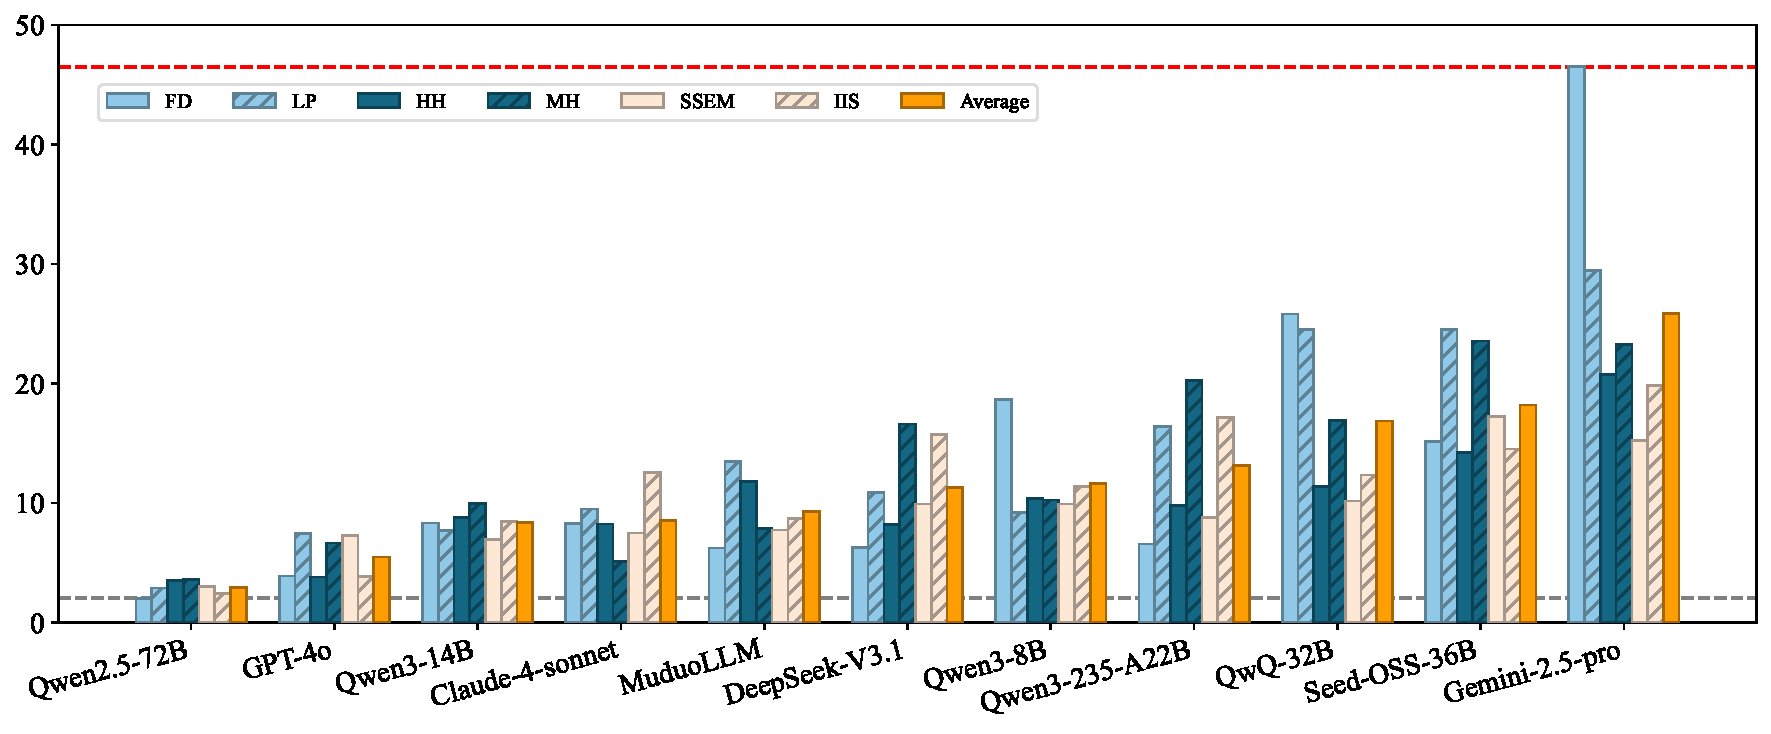
\includegraphics[height=0.41\textwidth]{figure/omnihardkd.pdf}
    \vspace{-5mm}
    \caption{Zero-shot average accuracy (\%) on the knowledge  dimension of OmniEduBench HARD.}
    \label{fig:omnihard_kd}
    \vspace{-3mm}
\end{figure}

\begin{figure}[tbp]
    \centering
    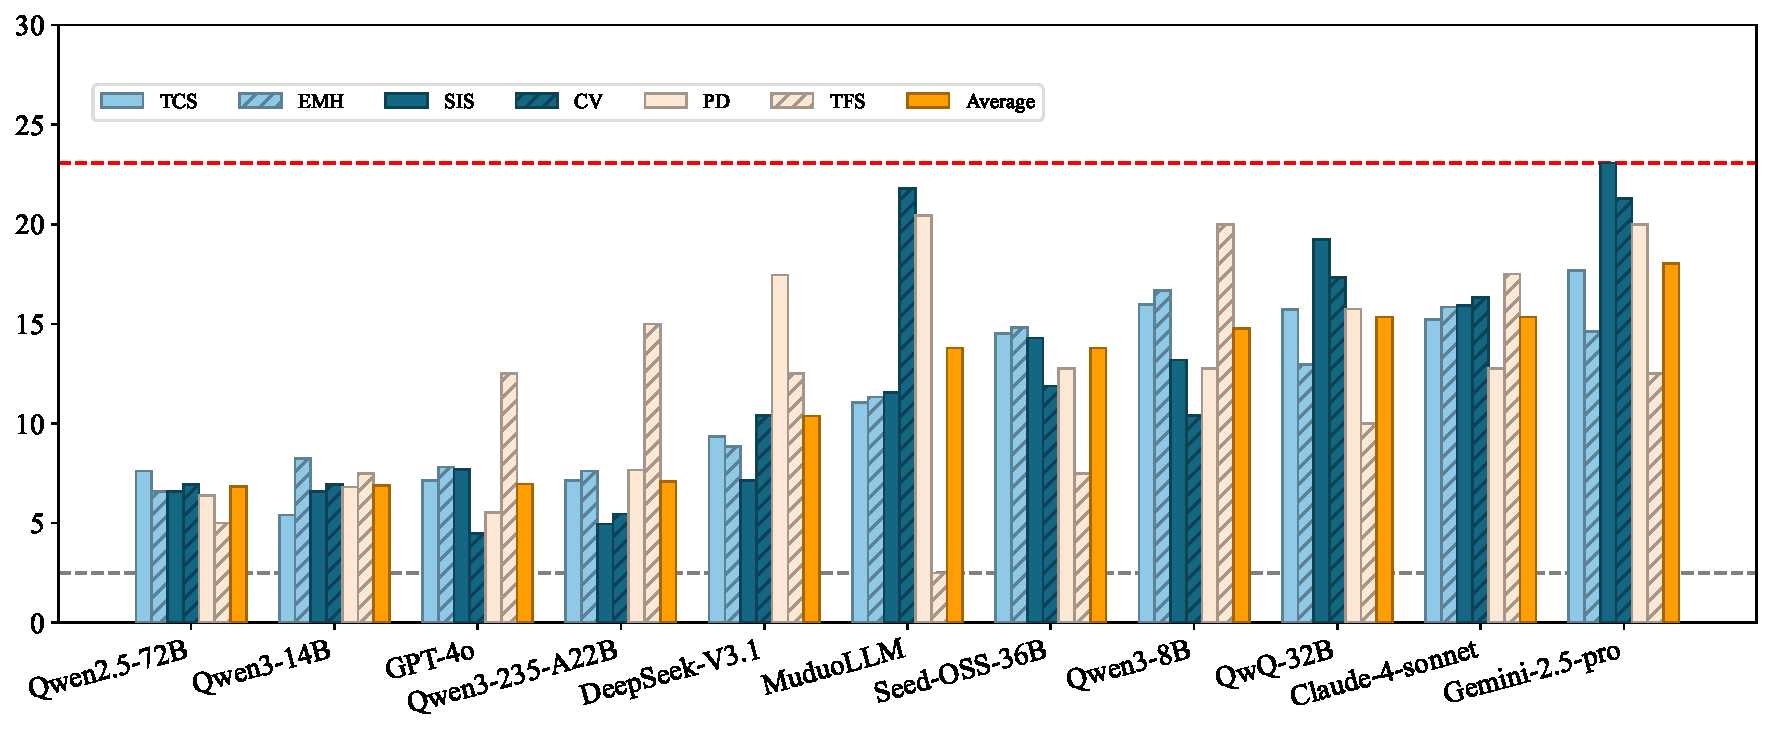
\includegraphics[height=0.41\textwidth]{figure/omnihardcd.pdf}
    \vspace{-5mm}
    \caption{Zero-shot average accuracy (\%) on the cultivation  dimension of OmniEduBench HARD.}
    \label{fig:omnihard_cd}
    \vspace{-3mm}
\end{figure}

\textbf{Results using different LLM-assisted scoring methods.}
In Table~\ref{tab:main_results_kd_llms}, we present the experimental results using different LLM-assisted scoring methods. The performance of the scoring model directly affects the evaluation outcomes: higher-quality scoring models provide more accurate assessments, leading to more precise measurements of the evaluated models’ capabilities. In this study, we employed three scoring models of varying quality. Overall, GPT-4o performed relatively poorly as a scoring model, failing to accurately evaluate the responses of LLMs. Consequently, the overall effectiveness of LLM-assisted evaluation is reduced when GPT-4o is used, highlighting the critical importance of selecting high-quality scoring models to ensure accurate and meaningful assessments. These findings suggest that the choice of scoring model can substantially influence the perceived performance of evaluated LLMs, and careful selection of scoring models is necessary.

\begin{table}[tbp]
    \centering
    \caption{Zero-shot average accuracy (\%) across six categories in the knowledge using different LLM-assisted scoring methods. The highest accuracy is \textbf{bold}, and the second highest is \underline{underlined}.}
    \vspace{0.2mm}
    \resizebox{0.99\textwidth}{!}{
        \begin{tabular}{lccc|cccccc|c}
            \toprule
            \textbf{Model} & \textbf{Parameters} & \textbf{Access} & \textbf{Creator} & \textbf{FD} & \textbf{HH} & \textbf{SSEM} & \textbf{LP} & \textbf{MH} & \textbf{IIS} & \textbf{Average} \\ \midrule
            \multicolumn{11}{c}{\textcolor{myorange}{\textit{Qwen3-A235B-assisted scoring method~\citep{yang2025qwen3}}}} \\
% Qwen3  & 8B & Weights & Alibaba & 55.45 & 48.51 & 42.54 & 30.86 & 38.13 & 44.42 & 48.85 \\
% Qwen3   & 14B & Weights & Alibaba & 37.82 & 48.70 & 40.60 & 29.07 & 38.45 & 41.14 & 40.76 \\
% MuduoLLM & 14B & Weights & BNU \& TAL & 27.78 & 43.22 & 34.08 & 36.01 & 39.00 & 29.21 & 34.18 \\
QwQ   & 32B & Weights& Alibaba & \underline{61.26} & 55.82 & 45.22 & \underline{50.10} & 55.66 & 48.36 & \underline{56.39} \\
Seed-OSS     & 36B &Weights & ByteDance & 51.16 & \underline{63.04} & \underline{51.55} & 50.38 & \textbf{62.31} & \underline{57.33} & 55.49 \\
% Qwen2.5 & 72B & Weights& Alibaba & 21.05 & 40.90 & 25.62 & 14.71 & 25.93 & 22.21 & 27.08 \\
% Qwen3   & 235B (22B active) & Weights & Alibaba & 37.11 & 59.20 & 42.97 & 45.77 & 61.00 & 53.61 & 46.85 \\
% DeepSeek-V3.1 & 671B (37B active) &Weights & DeepSeek & 29.94 & 40.47 & 33.72 & 29.42 & 50.33 & 41.36 & 34.93 \\
GPT-4o  & Undisclosed & API & OpenAI & 23.59 & 36.77 & 28.79 & 23.92 & 35.73 & 31.40 & 28.96 \\
Claude-4 Sonnet  & Undisclosed & API & Anthropic & 43.54 & 55.52 & 40.47 & 27.77 & 36.17 & 47.48 & 45.34 \\
Gemini-2.5 Pro  & Undisclosed & API & Google & \textbf{75.01} & \textbf{65.67} & \textbf{52.95} & \textbf{56.29} & \underline{61.44} & \textbf{61.49} & \textbf{67.41} \\
            \midrule
            \multicolumn{11}{c}{\textcolor{myorange}{\textit{Gemini-2.5 Pro-assisted scoring method~\citep{comanici2025gemini}}}} \\
% Qwen3  & 8B & Weights & Alibaba & 53.02 & 38.53 & 36.58 & 30.17 & 36.71 & 37.75 & 43.86 \\
% Qwen3   & 14B & Weights & Alibaba & 36.32 & 36.78 & 35.12 & 27.29 & 36.82 & 35.67 & 35.62 \\
% MuduoLLM & 14B & Weights & BNU \& TAL & 28.20 & 40.82 & 32.99 & 36.15 & 39.11 & 31.40 & 33.68 \\
QwQ   & 32B & Weights& Alibaba & \underline{61.25} & 48.51 & 42.24 & \underline{49.90} & 55.01 & 47.26 & \underline{53.87} \\
Seed-OSS     & 36B &Weights & ByteDance & 48.81 &\underline{50.14} & \underline{45.34} & 48.66 & \textbf{61.00} &\underline{49.56} & 49.53 \\
% Qwen2.5 & 72B & Weights& Alibaba & 19.53 & 30.95 & 20.57 & 13.26 & 23.86 & 20.90 & 22.76 \\
% Qwen3   & 235B (22B active) & Weights & Alibaba & 34.24 & 47.01 & 36.21 & 44.26 & 58.71 & 46.61 & 40.82 \\
% DeepSeek-V3.1 & 671B (37B active) &Weights & DeepSeek & 31.65 & 40.65 & 35.00 & 29.42 & 50.54 & 45.19 & 36.05 \\
GPT-4o  & Undisclosed & API & OpenAI & 21.15 & 26.94 & 23.92 & 22.13 & 34.75 & 27.13 & 24.17 \\
Claude-4 Sonnet  & Undisclosed & API & Anthropic & 41.49 & 44.29 & 35.36 & 27.56 & 34.86 & 42.34 & 40.35 \\
Gemini-2.5 Pro  & Undisclosed & API & Google & \textbf{73.83} & \textbf{55.13} & \textbf{46.68} & \textbf{55.40} & \underline{60.68} & \textbf{54.16} & \textbf{62.76} \\
            \midrule
            \multicolumn{11}{c}{\textcolor{myorange}{\textit{GPT-4o-assisted scoring method~\citep{hurst2024gpt-4o}}}} \\
% Qwen3  & 8B & Weights & Alibaba & 51.65 & 35.38 & 33.60 & 31.00 & 37.36 & 31.18 & 41.84 \\
% Qwen3   & 14B & Weights & Alibaba & 34.61 & 34.86 & 31.89 & 27.77 & 36.49 & 28.34 & 33.67 \\
% MuduoLLM & 14B & Weights & BNU \& TAL & 27.68 & 36.68 & 30.13 & 35.88 & 38.78 & 26.81 & 31.71 \\
QwQ   & 32B & Weights& Alibaba & \underline{56.61} & 42.87 & 37.86 & \underline{49.28} & 54.58 & 37.97 & \underline{49.26} \\
Seed-OSS     & 36B &Weights & ByteDance & 45.07 & \underline{47.89} & \underline{41.94} & 48.52 & \textbf{60.78} & \underline{43.54} & 46.61 \\
% Qwen2.5 & 72B & Weights& Alibaba & 18.60 & 27.53 & 18.50 & 11.41 & 23.20 & 15.75 & 20.72 \\
% Qwen3   & 235B (22B active) & Weights & Alibaba & 33.56 & 44.70 & 34.39 & 43.85 & 57.95 & 41.47 & 39.36 \\
% DeepSeek-V3.1 & 671B (37B active) &Weights & DeepSeek & 28.89 & 34.88 & 30.43 & 29.14 & 49.67 & 35.78 & 32.20 \\
GPT-4o  & Undisclosed & API & OpenAI & 20.38 & 23.78 & 22.03 & 22.06 & 34.31 & 23.30 & 22.51 \\
Claude-4 Sonnet  & Undisclosed & API & Anthropic & 40.43 & 41.70 & 31.89 & 27.90 & 35.08 & 34.79 & 38.48 \\
Gemini-2.5 Pro  & Undisclosed & API & Google & \textbf{70.15} & \textbf{51.38} & \textbf{44.13} & \textbf{55.88} & \underline{60.57} & \textbf{46.83} & \textbf{59.49} \\
            \bottomrule
        \end{tabular}}
    \label{tab:main_results_kd_llms}
    \vspace{-3mm}
\end{table}











% %  Hard部分知识维度
% \begin{table}[tbp]
%     \centering
%     \caption{Zero-shot average accuracy (\%) across six categories in the knowledge. The highest accuracy is \textbf{bold}, and the second highest is \underline{underlined}. More results are provided in the Appendix.}
%     \vspace{0.2mm}
%     \resizebox{0.99\textwidth}{!}{
%         \begin{tabular}{lccc|cccccc|c}
%             \toprule
%             \textbf{Model} & \textbf{Parameters} & \textbf{Access} & \textbf{Creator} & \textbf{FD} & \textbf{HH} & \textbf{SSEM} & \textbf{LP} & \textbf{MH} & \textbf{IIS} & \textbf{Average} \\ \midrule
% Qwen3  & 8B & Weights & Alibaba & 18.66 & 10.40 & 9.94 & 9.23 & 10.27 & 11.38 & 11.65 \\
% Qwen3   & 14B & Weights & Alibaba & 8.34 & 8.79 & 6.94 & 7.71 & 9.97 & 8.47 & 8.37 \\
% MuduoLLM & 14B & Weights & BNU \& TAL & 6.24 & 11.81 & 7.75 & 13.50 & 7.86 & 8.72 & 9.31 \\
% QwQ    & 32B & Weights & Alibaba & \underline{25.83} & 11.40 & 10.17 & \underline{24.52} & 16.92 & 12.35 & 16.86 \\
% Seed-OSS       & 36B & Weights & ByteDance & 15.17 & \underline{14.21} & \textbf{17.23} & \underline{24.52} & \textbf{23.57} & 14.53 & \underline{18.20} \\
% Qwen2.5 & 72B & Weights & Alibaba & 2.04 & 3.52 & 3.01 & 2.89 & 3.63 & 2.42 & 2.92 \\
% Qwen3   & 235B (22B active) & Weights & Alibaba & 6.58 & 9.82 & 8.79 & 16.39 & 20.24 & \underline{17.19} & 13.17 \\
% DeepSeek-V3.1 & 671B (37B active) & Weights & DeepSeek & 6.27 & 8.21 & 9.94 & 10.88 & 16.62 & 15.74 & 11.28 \\
% \midrule
% GPT-4o  & Undisclosed & API & OpenAI & 3.89 & 3.81 & 7.28 & 7.44 & 6.65 & 3.87 & 5.49 \\
% Claude-4 Sonnet  & Undisclosed & API & Anthropic & 8.28 & 8.25 & 7.51 & 9.50 & 5.14 & 12.59 & 8.55 \\
% Gemini-2.5 Pro  & Undisclosed & API & Google & \textbf{46.52} & \textbf{20.76} & \underline{15.26} & \textbf{29.48} & \underline{23.26} & \textbf{19.85} & \textbf{25.86} \\
%             \bottomrule
%         \end{tabular}}
%     \label{tab:main_results_kd_updated}
% \end{table}

% %  Hard部分育人维度
% \begin{table}[tbp]
%     \centering
%     \caption{Zero-shot average accuracy (\%) across six categories in the cultivation. The highest accuracy is \textbf{bold}, and the second highest is \underline{underlined}. More results are provided in the Appendix.}
%     \vspace{0.2mm}
%     \resizebox{0.99\textwidth}{!}{
%         \begin{tabular}{lccc|cccccc|c}
%             \toprule
%             \textbf{Model} & \textbf{Parameters} & \textbf{Access} & \textbf{Creator} & \textbf{TCS} & \textbf{EMH} & \textbf{SIS} & \textbf{CV} & \textbf{PD} & \textbf{TFS} & \textbf{Average} \\ \midrule
%             Qwen3 & 8B & Weights & Alibaba  & \underline{15.97} & \textbf{16.67} & 13.19 & 10.40 & 12.77 & \textbf{20.00} & 14.76 \\
%             Qwen3  & 14B & Weights & Alibaba & 5.41 & 8.23 & 6.59 & 6.93 & 6.81 & 7.50 & 6.89 \\
%             MuduoLLM  & 14B & Weights & BNU \& TAL & 11.06 & 11.32 & 11.54 & \textbf{21.78} & \textbf{20.43} & 2.50 & 13.79 \\
%             QwQ & 32B &Weights & Alibaba  & 15.72 & 12.96 & \underline{19.23} & 17.33 & 15.74 & 10.00 & \underline{15.34} \\
%             Seed\mbox{-}OSS & 36B &Weights & ByteDance & 14.50 & 14.81 & 14.29 & 11.88 & 12.77 & 7.50 & 13.79 \\
%             Qwen2.5 & 72B &Weights & Alibaba  & 7.62 & 6.58 & 6.59 & 6.93 & 6.38 & 5.00 & 6.83 \\
%             Qwen3 & 235B (22B active) &Weights & Alibaba & 7.13 & 7.61 & 4.95 & 5.45 & 7.66 & 15.00 & 7.09 \\
%             DeepSeek\mbox{-}V3.1  & 671B (37B active) &Weights& DeepSeek & 9.34 & 8.85 & 7.14 & 10.40 & 17.45 & 12.50 & 10.37 \\
%             \midrule
%             GPT\mbox{-}4o & Undisclosed & API & OpenAI & 7.13 & 7.82 & 7.69 & 4.46 & 5.53 & 12.50 & 6.96 \\
%             Claude\mbox{-}4\mbox{-}sonnet  & Undisclosed & API & Anthropic         & 15.23 & \underline{15.84} & 15.93 & 16.34 & 12.77 & \underline{17.50} & \underline{15.34} \\
%             Gemini\mbox{-}2.5\mbox{-}pro & Undisclosed & API & Google    & \textbf{17.69} & 14.61 & \textbf{23.08} & \underline{21.29} & \underline{20.00} & 12.50 & \textbf{18.04} \\
%             \bottomrule
%         \end{tabular}}
%     \label{tab:main_results_cd_updated}
% \end{table}